% answers.tex —— 1987 年·广东卷·文史类 · 参考答案与详细解析片段
% 由 tools/generate_projects.py 依来源总账自 1987/1987_数学真题_广东文_试题.md + 1987/1987_数学真题_广东文_解析正文.md + 1987/1987_数学真题_广东文_答案要点.md 生成，勿手改（改源 MD 后重跑）


\begin{gktip}
固定源题面与答案页覆盖第一卷、第二卷第一、二、四、五题；第三大题的固定源解答只交叉引用印刷页 286，本 PDF 未包含该页。第三大题以下推导为本库独立复算。
\end{gktip}

\begin{answer}
\gksolhead{1}{}

\textbf{题目}：

第一卷共 25 个选择题，每题只有一个结论正确。

（1） $\cos1030^\circ=$

（A）$\cos50^\circ$　　（B）$-\cos50^\circ$　　（C）$\sin50^\circ$　　（D）$-\sin50^\circ$

（2） $2^6$ 与 $0.5^2$ 的等比中项是

（A）$16$　　（B）$\pm4$　　（C）$2$　　（D）$4$

\Needspace{5\baselineskip}
（3） 函数

\nopagebreak[4]
\[
y=\sqrt{2x-x^2}
\]

的定义域是

（A）$(-\infty,0)$　　（B）$(0,2)$　　（C）$[0,2]$　　（D）$[-2,0]$

\Needspace{5\baselineskip}
（4） 指数方程

\nopagebreak[4]
\[
2\cdot4^x-5\cdot2^x+2=0
\]

的解集是

（A）$\{1\}$　　（B）$\{\frac12,1\}$　　（C）$\{-1,\frac12\}$　　（D）$\{-1,1\}$

（5） 下列不等式中，成立的是

（A）$\displaystyle\sin\frac{9\pi}{7}>\sin\frac{8\pi}{7}$

（B）$\displaystyle\cos\frac{9\pi}{7}>\cos\frac{8\pi}{7}$

（C）$\displaystyle\sec\frac{9\pi}{7}>\sec\frac{8\pi}{7}$

（D）$\displaystyle\operatorname{ctg}\frac{9\pi}{7}>\operatorname{ctg}\frac{8\pi}{7}$

（6） 如果圆锥的高和底面直径都等于 $a$，则该圆锥的体积是

（A）$\frac\pi4a^3$　　（B）$\frac\pi6a^3$　　（C）$\frac\pi3a^3$　　（D）$\frac\pi{12}a^3$

\Needspace{5\baselineskip}
（7） 在圆

\nopagebreak[4]
\[
x^2+y^2=4
\]

\Needspace{5\baselineskip}
上，与直线

\nopagebreak[4]
\[
4x+3y-12=0
\]

的距离最小的点的坐标是

（A）$\left(\frac85,\frac65\right)$　　（B）$\left(\frac85,-\frac65\right)$

（C）$\left(-\frac85,\frac65\right)$　　（D）$\left(-\frac85,-\frac65\right)$

（8） 若复数 $z$ 的辐角是 $\frac56\pi$，实部是 $-2\sqrt3$，则 $z=$

（A）$-2\sqrt3-2i$　　（B）$-2\sqrt3+2i$

（C）$-2\sqrt3+2\sqrt3\,i$　　（D）$-2\sqrt3-2\sqrt3\,i$

\Needspace{5\baselineskip}
（9） 已知函数

\nopagebreak[4]
\[
f(x)=x^{\frac13},\qquad g(x)=\left(\frac13\right)^x,
\]

那么，在 $(-\infty,+\infty)$ 上，

（A）$f(x)$ 和 $g(x)$ 都是增函数。

（B）$f(x)$ 和 $g(x)$ 都是减函数。

（C）$f(x)$ 是减函数，而 $g(x)$ 是增函数。

（D）$f(x)$ 是增函数，而 $g(x)$ 是减函数。

\Needspace{5\baselineskip}
（10） 计算下式：

\nopagebreak[4]
\[
\frac{(\sin\alpha+\cos\alpha)^2-(\sin\alpha-\cos\alpha)^2}
{\operatorname{tg}\alpha-\sin\alpha\cos\alpha}
=
\]

（A）$2\operatorname{ctg}^2\alpha$　　（B）$2\operatorname{tg}^2\alpha$

（C）$4\operatorname{ctg}^2\alpha$　　（D）$4\operatorname{tg}^2\alpha$

\Needspace{5\baselineskip}
（11） 函数

\nopagebreak[4]
\[
y=\sin3x+2\cos3x
\]

的最小值是

（A）$-2$　　（B）$-\sqrt5$　　（C）$-3$　　（D）$-5$

\Needspace{5\baselineskip}
（12） 若

\nopagebreak[4]
\[
\operatorname{ctg}\frac\theta2=3,
\]

则 $\cos\theta$ 的值是

（A）$\frac35$　　（B）$-\frac35$　　（C）$-\frac45$　　（D）$\frac45$

\Needspace{5\baselineskip}
（13） 不等式

\nopagebreak[4]
\[
\frac{3x-1}{2-x}\geq1
\]

的解集是

（A）$\left\{x\mid\frac34\leq x\leq2\right\}$

（B）$\left\{x\mid\frac34\leq x<2\right\}$

（C）$\left\{x\mid x>2\ \mathrm{or}\ x\leq\frac34\right\}$

（D）$\{x\mid x<2\}$

\Needspace{5\baselineskip}
（14） 设

\nopagebreak[4]
\[
f(x)=\frac{2x+1}{4x+3}\qquad(x\in R,\ x\ne-\frac34),
\]

\Needspace{5\baselineskip}
则

\nopagebreak[4]
\[
f^{-1}(2)=
\]

（A）$-\frac56$　　（B）$\frac5{11}$　　（C）$\frac25$　　（D）$-\frac25$

（15） 用 $0,1,2,3$ 这四个数字，组成个位数不是 1 的没有重复数字的四位数，共有

（A）16 个　　（B）14 个　　（C）12 个　　（D）10 个

\Needspace{5\baselineskip}
（16） 抛物线

\nopagebreak[4]
\[
y=x^2+3x-2
\]

的对称轴的方程是

（A）$x=\sqrt3$　　（B）$x=-\sqrt3$　　（C）$x=\frac32$　　（D）$x=-\frac32$

\Needspace{5\baselineskip}
（17） 设 $A,B$ 是直线

\nopagebreak[4]
\[
3x+4y+2=0
\]

\Needspace{5\baselineskip}
与圆

\nopagebreak[4]
\[
x^2+y^2+4y=0
\]

的两个交点，则线段 $AB$ 的垂直平分线的方程是

（A）$3y-4x+2=0$　　（B）$3y-4x+6=0$

（C）$3y+4x+6=0$　　（D）$4y+3x+8=0$

\Needspace{5\baselineskip}
（18） 椭圆

\nopagebreak[4]
\[
x^2+4y^2+4x=0
\]

的右焦点的坐标是

（A）$(\sqrt3-2,0)$　　（B）$(\sqrt3+2,0)$

（C）$(\sqrt3,0)$　　（D）$(-\sqrt3,0)$

（19） 设双曲线的半焦距为 $c$，两条准线的距离为 $d$，且 $c=d$，则这双曲线的离心率 $e=$

（A）$\sqrt3$　　（B）$\sqrt2$　　（C）$2$　　（D）$3$

\Needspace{5\baselineskip}
（20） 若

\nopagebreak[4]
\[
\theta\in\left(\frac\pi2,\frac34\pi\right),
\]

\Needspace{5\baselineskip}
则

\nopagebreak[4]
\[
\frac{x^2}{\csc\theta-2}+\frac{y^2}{2-\sec\theta}=1
\]

所表示的曲线是

（A）焦点在 $x$ 轴上的椭圆。

（B）焦点在 $y$ 轴上的椭圆。

（C）焦点在 $x$ 轴上的双曲线。

（D）焦点在 $y$ 轴上的双曲线。

（21） 若正三棱锥的一个侧面的面积与底面的面积的比等于 $\frac23$，则这个三棱锥的侧面和底面所成的二面角是

（A）$15^\circ$　　（B）$30^\circ$　　（C）$45^\circ$　　（D）$60^\circ$

（22） 设 $\alpha$ 和 $\beta$ 是两个不重合的平面，$l$ 和 $m$ 是两条不重合的直线，则 $\alpha\parallel\beta$ 的一个充分条件是

（A）$l\subset\alpha,\ m\subset\alpha$，且 $l\parallel\beta,\ m\parallel\beta$。

（B）$l\subset\alpha,\ m\subset\beta$，且 $l\parallel m$。

（C）$l\perp\alpha,\ m\perp\beta$，且 $l\parallel m$。

（D）$l\parallel\alpha,\ m\parallel\beta$，且 $l\parallel m$。

（23） 如果实数 $a,b,c$ 不全为零，那么

（A）实数 $a,b,c$ 中，至少有一个正数。

（B）实数 $a,b,c$ 中，既有正数又有负数。

（C）实数 $a,b,c$ 的乘积不是零。

（D）实数 $a,b,c$ 中，至多有两个零。

\Needspace{5\baselineskip}
（24） 已知函数

\nopagebreak[4]
\[
f(x)=\sin\left(\frac34x+\frac52\pi\right),
\qquad
g(x)=\lg\left(\sqrt{x^2+1}-x\right),
\]

则

（A）$f(x)$ 是奇函数，而 $g(x)$ 既不是奇函数，又不是偶函数。

（B）$f(x)$ 是偶函数，而 $g(x)$ 是奇函数。

（C）$f(x)$ 和 $g(x)$ 都是奇函数。

（D）$f(x)$ 是偶函数，而 $g(x)$ 既不是奇函数，又不是偶函数。

\Needspace{5\baselineskip}
（25） 若等差数列的第一、二、三项依次是

\nopagebreak[4]
\[
\frac1{x+1},\qquad \frac5{6x},\qquad \frac1x,
\]

那么，这个等差数列的第 101 项的值是

（A）$50\frac13$　　（B）$13\frac23$　　（C）$24$　　（D）$8\frac23$

\Needspace{4\baselineskip}
\textbf{解析}

\gksubpart{（1）}

\Needspace{5\baselineskip}
因为 $1030^\circ=2\cdot360^\circ+310^\circ$，所以

\nopagebreak[4]
\[
\cos1030^\circ=\cos310^\circ=\cos50^\circ.
\]

答案为 A。

\gksubpart{（2）}

\Needspace{4\baselineskip}
\textbf{解析}

\Needspace{5\baselineskip}
设等比中项为 $u$，则

\nopagebreak[4]
\[
u^2=2^6\cdot0.5^2=16.
\]

所以 $u=\pm4$，答案为 B。

\gksubpart{（3）}

\Needspace{4\baselineskip}
\textbf{解析}

\Needspace{5\baselineskip}
根式有意义要求 $2x-x^2\ge0$，即

\nopagebreak[4]
\[
x(2-x)\ge0.
\]

所以定义域为 $[0,2]$，答案为 C。

\gksubpart{（4）}

\Needspace{4\baselineskip}
\textbf{解析}

\Needspace{5\baselineskip}
令 $t=2^x>0$，原方程化为

\nopagebreak[4]
\[
2t^2-5t+2=0.
\]

解得 $t=1/2$ 或 $t=2$，即 $x=-1$ 或 $x=1$。答案为 D。

\gksubpart{（5）}

\Needspace{4\baselineskip}
\textbf{解析}

\Needspace{5\baselineskip}
有

\nopagebreak[4]
\[
\cos\frac{9\pi}{7}=-\cos\frac{2\pi}{7},
\qquad
\cos\frac{8\pi}{7}=-\cos\frac{\pi}{7}.
\]

由于 $\cos(2\pi/7)<\cos(\pi/7)$，故选项 B 成立。

\gksubpart{（6）}

\Needspace{4\baselineskip}
\textbf{解析}

\Needspace{5\baselineskip}
圆锥底面半径为 $a/2$，高为 $a$，故

\nopagebreak[4]
\[
V=\frac13\pi\left(\frac a2\right)^2a=\frac\pi{12}a^3.
\]

答案为 D。

\gksubpart{（7）}

\Needspace{4\baselineskip}
\textbf{解析}

\Needspace{5\baselineskip}
圆心为原点，半径为 $2$。使点到直线的距离最小，就是使 $4x+3y$ 在圆上取得最大值，故点为

\nopagebreak[4]
\[
2\frac{(4,3)}5=\left(\frac85,\frac65\right).
\]

答案为 A。

\gksubpart{（8）}

\Needspace{4\baselineskip}
\textbf{解析}

\Needspace{5\baselineskip}
辐角为 $5\pi/6$ 时，复数位于第二象限。由实部 $-2\sqrt3$ 和

\nopagebreak[4]
\[
\tan\frac{5\pi}{6}=-\frac1{\sqrt3}
\]

得虚部为 $2$，所以 $z=-2\sqrt3+2i$。答案为 B。

\gksubpart{（9）}

\Needspace{4\baselineskip}
\textbf{解析}

$x^{1/3}$ 在实数集上递增，而底数 $1/3$ 的指数函数递减，答案为 D。

\gksubpart{（10）}

\Needspace{4\baselineskip}
\textbf{解析}

\Needspace{5\baselineskip}
分子为

\nopagebreak[4]
\[
(\sin\alpha+\cos\alpha)^2-(\sin\alpha-\cos\alpha)^2
=4\sin\alpha\cos\alpha.
\]

\Needspace{5\baselineskip}
分母为

\nopagebreak[4]
\[
\tan\alpha-\sin\alpha\cos\alpha
=\frac{\sin^3\alpha}{\cos\alpha}.
\]

因此原式等于 $4\operatorname{ctg}^2\alpha$，答案为 C。

\gksubpart{（11）}

\Needspace{4\baselineskip}
\textbf{解析}

\Needspace{5\baselineskip}
函数的振幅为

\nopagebreak[4]
\[
\sqrt{1^2+2^2}=\sqrt5.
\]

所以最小值为 $-\sqrt5$，答案为 B。

\gksubpart{（12）}

\Needspace{4\baselineskip}
\textbf{解析}

\Needspace{5\baselineskip}
由 $\operatorname{ctg}(\theta/2)=3$ 得 $\tan(\theta/2)=1/3$，从而

\nopagebreak[4]
\[
\cos\theta=\frac{1-\tan^2(\theta/2)}{1+\tan^2(\theta/2)}
=\frac45.
\]

答案为 D。

\gksubpart{（13）}

\Needspace{4\baselineskip}
\textbf{解析}

\nopagebreak[4]
\[
\frac{3x-1}{2-x}-1=\frac{4x-3}{2-x}\ge0.
\]

作符号分析得解集为 $[3/4,2)$，答案为 B。

\gksubpart{（14）}

\Needspace{4\baselineskip}
\textbf{解析}

\Needspace{5\baselineskip}
由 $f(x)=2$ 得

\nopagebreak[4]
\[
\frac{2x+1}{4x+3}=2
\Longrightarrow x=-\frac56.
\]

答案为 A。

\gksubpart{（15）}

\Needspace{4\baselineskip}
\textbf{解析}

个位为 $0$ 时，千位有 $3$ 种选法，其余两位有 $2$ 种排法，共 $6$ 个。个位为 $2$ 或 $3$ 时，千位各有 $2$ 种选法，其余两位各有 $2$ 种排法，共 $4+4$ 个。

总数为 $6+4+4=14$，答案为 B。

\gksubpart{（16）}

\Needspace{4\baselineskip}
\textbf{解析}

\Needspace{5\baselineskip}
二次函数的对称轴为

\nopagebreak[4]
\[
x=-\frac{3}{2},
\]

答案为 D。

\gksubpart{（17）}

\Needspace{4\baselineskip}
\textbf{解析}

\Needspace{5\baselineskip}
圆心为 $(0,-2)$，弦 $AB$ 所在直线斜率为 $-3/4$，其垂直平分线斜率为 $4/3$，且经过圆心。因此方程为

\nopagebreak[4]
\[
y+2=\frac43x,
\qquad
3y-4x+6=0.
\]

答案为 B。

\gksubpart{（18）}

\Needspace{4\baselineskip}
\textbf{解析}

\Needspace{5\baselineskip}
配方得

\nopagebreak[4]
\[
(x+2)^2+4y^2=4.
\]

\Needspace{5\baselineskip}
所以椭圆的半长轴为 $2$，半短轴为 $1$，焦距参数为 $\sqrt3$。右焦点为

\nopagebreak[4]
\[
(\sqrt3-2,0),
\]

答案为 A。

\gksubpart{（19）}

\Needspace{4\baselineskip}
\textbf{解析}

\Needspace{5\baselineskip}
双曲线的两条准线距离为 $d=2a/e$，半焦距为 $c=ae$。由 $c=d$ 得

\nopagebreak[4]
\[
ae=\frac{2a}{e},
\qquad e^2=2.
\]

故 $e=\sqrt2$，答案为 B。

\gksubpart{（20）}

\Needspace{4\baselineskip}
\textbf{解析}

\Needspace{5\baselineskip}
当 $\theta\in(\pi/2,3\pi/4)$ 时，$\csc\theta<2$ 且 $\sec\theta<0$，所以

\nopagebreak[4]
\[
\csc\theta-2<0,\qquad 2-\sec\theta>0.
\]

方程表示焦点在 $y$ 轴上的双曲线，答案为 D。

\gksubpart{（21）}

\Needspace{4\baselineskip}
\textbf{解析}

\Needspace{5\baselineskip}
设正三棱锥底边长为 $a$，侧面斜高为 $l$。面积比给出

\nopagebreak[4]
\[
\frac{\frac12al}{\frac{\sqrt3}{4}a^2}=\frac23,
\qquad
l=\frac a{\sqrt3}.
\]

底面中心到边中点的距离为 $a\sqrt3/6$，于是三棱锥高为 $a/2$，二面角的正切为 $\sqrt3$，故二面角为 $60^\circ$。答案为 D。

\gksubpart{（22）}

\Needspace{4\baselineskip}
\textbf{解析}

若 $l\perp\alpha$、$m\perp\beta$ 且 $l\parallel m$，则 $\alpha$、$\beta$ 的法向方向平行。由于两平面不重合，必有 $\alpha\parallel\beta$，答案为 C。

\gksubpart{（23）}

\Needspace{4\baselineskip}
\textbf{解析}

“不全为零”表示至少有一个数非零，所以零的个数至多为 $2$，答案为 D。

\gksubpart{（24）}

\Needspace{4\baselineskip}
\textbf{解析}

\nopagebreak[4]
\[
f(x)=\sin\left(\frac34x+\frac52\pi\right)
=\cos\frac34x,
\]

\Needspace{5\baselineskip}
所以 $f$ 为偶函数。又

\nopagebreak[4]
\[
\left(\sqrt{x^2+1}-x\right)\left(\sqrt{x^2+1}+x\right)=1,
\]

从而 $g(-x)=-g(x)$，即 $g$ 为奇函数。答案为 B。

\gksubpart{（25）}

\Needspace{4\baselineskip}
\textbf{解析}

\Needspace{5\baselineskip}
等差条件为

\nopagebreak[4]
\[
2\cdot\frac5{6x}=\frac1{x+1}+\frac1x.
\]

\Needspace{5\baselineskip}
解得 $x=2$。于是首项为 $1/3$，公差为 $1/12$，故

\nopagebreak[4]
\[
a_{101}=\frac13+100\cdot\frac1{12}
=\frac{26}{3}=8\frac23.
\]

答案为 D。

\gkanswer{答案（1）：A}

\gkanswer{答案（2）：B}

\gkanswer{答案（3）：C}

\gkanswer{答案（4）：D}

\gkanswer{答案（5）：B}

\gkanswer{答案（6）：D}

\gkanswer{答案（7）：A}

\gkanswer{答案（8）：B}

\gkanswer{答案（9）：D}

\gkanswer{答案（10）：C}

\gkanswer{答案（11）：B}

\gkanswer{答案（12）：D}

\gkanswer{答案（13）：B}

\gkanswer{答案（14）：A}

\gkanswer{答案（15）：B}

\gkanswer{答案（16）：D}

\gkanswer{答案（17）：B}

\gkanswer{答案（18）：A}

\gkanswer{答案（19）：B}

\gkanswer{答案（20）：D}

\gkanswer{答案（21）：D}

\gkanswer{答案（22）：C}

\gkanswer{答案（23）：D}

\gkanswer{答案（24）：B}

\gkanswer{答案（25）：D}

\end{answer}
\begin{answer}
\gksolhead{2}{}

\textbf{题目}：

第二卷第一题（本题满分 15 分）共有五个填空小题，每小题 3 分。

\Needspace{5\baselineskip}
（1） 若

\nopagebreak[4]
\[
z=\sqrt2+i,
\]

则 $z^2$ 的共轭复数的代数形式是 $\underline{\hspace{3em}}$。

（2） 已知椭圆的两个焦点是 $F_1(-2,0),F_2(2,0)$，并且点 $A(0,2)$ 在该椭圆上，那么，这个椭圆的标准方程是 $\underline{\hspace{5em}}$。

\Needspace{5\baselineskip}
（3） 计算极限：

\nopagebreak[4]
\[
\lim_{n\to\infty}\frac{4n^3-1}{n(2n^2+1)}
\]

的值是 $\underline{\hspace{3em}}$。

\Needspace{5\baselineskip}
（4） 设

\nopagebreak[4]
\[
(1-x)^7=a_0+a_1x+a_2x^2+a_3x^3+a_4x^4+a_5x^5+a_6x^6+a_7x^7,
\]

\Needspace{5\baselineskip}
则

\nopagebreak[4]
\[
a_0+a_2+a_4+a_6
\]

的值是 $\underline{\hspace{3em}}$。

\Needspace{5\baselineskip}
（5） 函数

\nopagebreak[4]
\[
y=\frac{2x}{1+x^2}\qquad(x\in R)
\]

的值域是 $\underline{\hspace{3em}}$。

\Needspace{4\baselineskip}
\textbf{解析}

\gksubpart{（1）}

\nopagebreak[4]
\[
z^2=(\sqrt2+i)^2=1+2\sqrt2\,i,
\]

\Needspace{5\baselineskip}
所以

\nopagebreak[4]
\[
\overline{z^2}=1-2\sqrt2\,i.
\]

\gksubpart{（2）}

\Needspace{4\baselineskip}
\textbf{解析}

\Needspace{5\baselineskip}
椭圆半焦距为 $c=2$，点 $(0,2)$ 在椭圆上，因此短半轴为 $b=2$。由 $a^2=b^2+c^2$ 得 $a^2=8$，标准方程为

\nopagebreak[4]
\[
\frac{x^2}{8}+\frac{y^2}{4}=1.
\]

\gksubpart{（3）}

\Needspace{4\baselineskip}
\textbf{解析}

\nopagebreak[4]
\[
\lim_{n\to\infty}\frac{4n^3-1}{n(2n^2+1)}
=\lim_{n\to\infty}\frac{4-n^{-3}}{2+n^{-1}}
=2.
\]

\gksubpart{（4）}

\Needspace{4\baselineskip}
\textbf{解析}

\Needspace{5\baselineskip}
偶次幂系数和为

\nopagebreak[4]
\[
\frac{(1-1)^7+(1+1)^7}{2}=64.
\]

\gksubpart{（5）}

\Needspace{4\baselineskip}
\textbf{解析}

\Needspace{5\baselineskip}
由

\nopagebreak[4]
\[
1-\frac{2x}{1+x^2}=\frac{(x-1)^2}{1+x^2}\ge0,
\qquad
1+\frac{2x}{1+x^2}=\frac{(x+1)^2}{1+x^2}\ge0,
\]

可知 $-1\le y\le1$，且两端均可取到，值域为 $[-1,1]$。

\gkanswer{答案（1）：$1-2\sqrt2\,i$}

\gkanswer{答案（2）：$\displaystyle\frac{x^2}{8}+\frac{y^2}{4}=1$}

\gkanswer{答案（3）：$2$}

\gkanswer{答案（4）：$64$}

\gkanswer{答案（5）：$[-1,1]$}

\end{answer}
\begin{answer}
\gksolhead{3}{}

\textbf{题目}：

\Needspace{5\baselineskip}
第二卷第二题（本题满分 12 分）。设正数 $a,b,c$ 满足

\nopagebreak[4]
\[
a^2+b^2=c^2.
\]

\Needspace{5\baselineskip}
（1） 求证：

\nopagebreak[4]
\[
\log_2\left(1+\frac{b+c}{a}\right)
+\log_2\left(1+\frac{a-c}{b}\right)=1.
\]

\Needspace{5\baselineskip}
（2） 又设

\nopagebreak[4]
\[
\log_4\left(1+\frac{b+c}{a}\right)=1,\qquad
\log_8(a+b-c)=\frac23,
\]

求 $a,b,c$ 的值。

\Needspace{4\baselineskip}
\textbf{解析}

\gksubpart{（1）}

\Needspace{5\baselineskip}
由 $a^2+b^2=c^2$，

\nopagebreak[4]
\[
\left(1+\frac{b+c}{a}\right)
\left(1+\frac{a-c}{b}\right)
=\frac{(a+b+c)(a+b-c)}{ab}
=\frac{(a+b)^2-c^2}{ab}=2.
\]

两个对数真数均为正，故对数相加等于 $\log_2 2=1$。

\gksubpart{（2）}

\Needspace{4\baselineskip}
\textbf{解析}

\Needspace{5\baselineskip}
由第一个对数条件得

\nopagebreak[4]
\[
1+\frac{b+c}{a}=4,
\qquad b+c=3a.
\]

\Needspace{5\baselineskip}
由第二个条件得

\nopagebreak[4]
\[
a+b-c=4.
\]

\Needspace{5\baselineskip}
消去 $c$ 得 $b=a+2$、$c=2a-2$。代入 $a^2+b^2=c^2$，得 $a=6$，从而

\nopagebreak[4]
\[
b=8,\qquad c=10.
\]

\gkanswer{答案（1）：$1$}

\gkanswer{答案（2）：$a=6,\ b=8,\ c=10$}

\end{answer}
\begin{answer}
\gksolhead{4}{}

\textbf{题目}：

\Needspace{5\baselineskip}
第二卷第三题（本题满分 14 分）。在三棱台

\nopagebreak[4]
\[
A_1B_1C_1-ABC
\]

\Needspace{5\baselineskip}
中，侧棱 $B_1B\perp$ 底面 $ABC$，且

\nopagebreak[4]
\[
\angle ABC=\angle AA_1C=\frac\pi2,\qquad
AB=2A_1B_1=2\text{ cm}.
\]
\nopagebreak[4]
\begin{center}% 1987 年广东卷文史类第三大题：三棱台
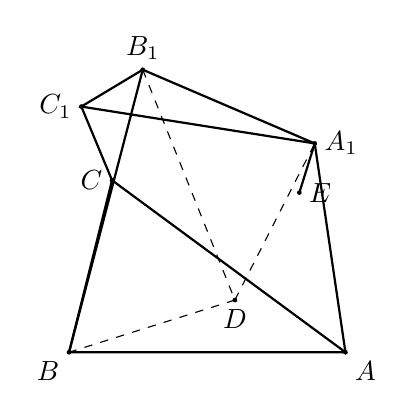
\begin{tikzpicture}[scale=0.78,>=stealth]
  \coordinate (A) at (4.5,0);
  \coordinate (B) at (0,0);
  \coordinate (C) at (0.7,2.8);
  \coordinate (A1) at (4.0,3.4);
  \coordinate (B1) at (1.2,4.6);
  \coordinate (C1) at (0.2,4.0);
  \coordinate (D) at (2.7,0.85);
  \coordinate (E) at (3.75,2.6);
  \draw[thick] (A)--(B)--(C)--(A);
  \draw[thick] (A1)--(B1)--(C1)--(A1);
  \draw[thick] (A)--(A1) (B)--(B1) (C)--(C1);
  \draw[dashed] (B1)--(D) (D)--(A1) (D)--(B);
  \draw[thick] (E)--(A1);
  \fill (A) circle (1.1pt) node[below right] {$A$};
  \fill (B) circle (1.1pt) node[below left] {$B$};
  \fill (C) circle (1.1pt) node[left] {$C$};
  \fill (A1) circle (1.1pt) node[right] {$A_1$};
  \fill (B1) circle (1.1pt) node[above] {$B_1$};
  \fill (C1) circle (1.1pt) node[left] {$C_1$};
  \fill (D) circle (1.1pt) node[below] {$D$};
  \fill (E) circle (1.1pt) node[right] {$E$};
\end{tikzpicture}
\end{center}
\nopagebreak[4]
（1） 求证：$BC\perp A_1B,\ BC\perp A_1A,\ A_1A\perp A_1B$。

（2） 求异面直线 $A_1A$ 和 $BC$ 的距离。

\Needspace{4\baselineskip}
\textbf{解析}

\gksubpart{（1）}

固定源本 PDF 对本题只给出“解答见印刷页 286”的交叉引用，未提供本题固定源解答。以下为独立推导。

\Needspace{5\baselineskip}
取

\nopagebreak[4]
\[
B=(0,0,0),\quad A=(2,0,0),\quad C=(0,s,0).
\]

\Needspace{5\baselineskip}
由两底面平行、$AB=2$、$A_1B_1=1$ 及 $B_1B\perp$ 底面，可设

\nopagebreak[4]
\[
B_1=(0,0,h),\qquad A_1=(1,0,h).
\]

\Needspace{5\baselineskip}
条件 $\angle AA_1C=\pi/2$ 给出

\nopagebreak[4]
\[
(A-A_1)\cdot(C-A_1)
=(1,0,-h)\cdot(-1,s,-h)=h^2-1=0,
\]

\Needspace{5\baselineskip}
所以 $h=1$。于是

\nopagebreak[4]
\[
\overrightarrow{BC}=(0,s,0),\quad
\overrightarrow{A_1B}=(-1,0,-1),\quad
\overrightarrow{A_1A}=(1,0,-1).
\]

\Needspace{5\baselineskip}
三组向量的内积分别为零，故

\nopagebreak[4]
\[
BC\perp A_1B,\qquad
BC\perp A_1A,\qquad
A_1A\perp A_1B.
\]

\gksubpart{（2）}

\Needspace{4\baselineskip}
\textbf{解析}

\Needspace{5\baselineskip}
$A_1B$ 同时垂直于 $BC$ 和 $A_1A$，是两条异面直线的公垂线。因此

\nopagebreak[4]
\[
d(A_1A,BC)=|A_1B|=\sqrt{1^2+1^2}=\sqrt2\text{ cm}.
\]

\gkanswer{答案（1）：本固定源仅交叉引用印刷页 286；独立推导见解析正文。}

\gkanswer{答案（2）：$\sqrt2\text{ cm}$（独立推导）}

\end{answer}
\begin{answer}
\gksolhead{5}{}

\textbf{题目}：

\Needspace{5\baselineskip}
第二卷第四题（本题满分 15 分）。直线 $l$ 通过抛物线

\nopagebreak[4]
\[
y^2=2px\qquad(p\ne0)
\]

的焦点，并且与这抛物线相交于 $A(x_1,y_1)$ 和 $B(x_2,y_2)$ 两点。

\Needspace{5\baselineskip}
（1） 求证：

\nopagebreak[4]
\[
y_1y_2=-p^2.
\]

（2） 点 $C$ 在这条抛物线的准线上，且 $AC$ 平行于 $x$ 轴，求证：$B,C$ 和这条抛物线的顶点三点共线。

\Needspace{4\baselineskip}
\textbf{解析}

\gksubpart{（1）}

\Needspace{5\baselineskip}
抛物线焦点为 $F(p/2,0)$。若直线 $l$ 垂直于 $x$ 轴，则交点纵坐标为 $\pm p$，结论立即成立。否则设

\nopagebreak[4]
\[
y=k\left(x-\frac p2\right).
\]

\Needspace{5\baselineskip}
代入 $y^2=2px$，得到

\nopagebreak[4]
\[
y^2-\frac{2p}{k}y-p^2=0.
\]

\Needspace{5\baselineskip}
其两个根为 $y_1,y_2$，故

\nopagebreak[4]
\[
y_1y_2=-p^2.
\]

\gksubpart{（2）}

\Needspace{4\baselineskip}
\textbf{解析}

\Needspace{5\baselineskip}
抛物线准线为 $x=-p/2$。由于 $AC$ 平行于 $x$ 轴，

\nopagebreak[4]
\[
C=\left(-\frac p2,y_1\right).
\]

\Needspace{5\baselineskip}
又 $B=(y_2^2/(2p),y_2)$，所以

\nopagebreak[4]
\[
\frac{y_2}{x_B}
=\frac{2p}{y_2}
=-\frac{2y_1}{p}
=\frac{y_1}{-p/2}.
\]

这说明 $OB$ 与 $OC$ 斜率相同，故 $B,C$ 和抛物线顶点 $O$ 三点共线。

\gkanswer{答案（1）：$y_1y_2=-p^2$}

\gkanswer{答案（2）：$B,C$ 与抛物线顶点三点共线}

\end{answer}
\begin{answer}
\gksolhead{6}{}

\textbf{题目}：

\Needspace{5\baselineskip}
第二卷第五题（本题满分 14 分）。设 $|\theta|<\frac\pi2$，数列 $\{a_n\}$ 的通项是

\nopagebreak[4]
\[
a_n=\sin\frac{n\pi}{2}\cdot\operatorname{tg}^n\theta,
\]

\Needspace{5\baselineskip}
记

\nopagebreak[4]
\[
S_{2n}=a_1+a_2+\cdots+a_{2n-1}+a_{2n}.
\]

\Needspace{5\baselineskip}
（1） 求证：对任何自然数 $n$，

\nopagebreak[4]
\[
S_{2n}=\frac12(\sin2\theta)
\left[1+(-1)^{n+1}\operatorname{tg}^{2n}\theta\right].
\]

\Needspace{5\baselineskip}
（2） 求证：当 $n\ge2$ 时，

\nopagebreak[4]
\[
a_n^2+a_{n-1}\cdot a_{n+1}+(-1)^n(a_1)^{2n}=0.
\]

\Needspace{4\baselineskip}
\textbf{解析}

\gksubpart{（1）}

\Needspace{5\baselineskip}
令 $t=\operatorname{tg}\theta$，则

\nopagebreak[4]
\[
a_{2j}=0,\qquad a_{2j-1}=(-1)^{j+1}t^{2j-1}.
\]

\Needspace{5\baselineskip}
因此

\nopagebreak[4]
\[
S_{2n}=t-t^3+\cdots+(-1)^{n+1}t^{2n-1}
=\frac{t}{1+t^2}\left[1+(-1)^{n+1}t^{2n}\right].
\]

由于 $t/(1+t^2)=\frac12\sin2\theta$，得到题中结论。

\gksubpart{（2）}

\Needspace{4\baselineskip}
\textbf{解析}

\Needspace{5\baselineskip}
当 $n$ 为偶数时，$a_n=0$，且

\nopagebreak[4]
\[
a_{n-1}a_{n+1}=-t^{2n},
\qquad
(-1)^n(a_1)^{2n}=t^{2n}.
\]

\Needspace{5\baselineskip}
当 $n$ 为奇数时，$a_{n-1}a_{n+1}=0$，且

\nopagebreak[4]
\[
a_n^2=t^{2n},
\qquad
(-1)^n(a_1)^{2n}=-t^{2n}.
\]

\Needspace{5\baselineskip}
两种情形均有

\nopagebreak[4]
\[
a_n^2+a_{n-1}a_{n+1}+(-1)^n(a_1)^{2n}=0.
\]

\gkanswer{答案（1）：$\displaystyle S_{2n}=\frac12(\sin2\theta)\left[1+(-1)^{n+1}\operatorname{tg}^{2n}\theta\right]$}

\gkanswer{答案（2）：$\displaystyle a_n^2+a_{n-1}a_{n+1}+(-1)^n(a_1)^{2n}=0$}

\end{answer}